%
% File tupa_amr.tex

\documentclass[11pt,a4paper]{article}
\usepackage[hyperref]{conll2018}
\usepackage{times}
\usepackage{latexsym}
\usepackage{tikz}
\usepackage{tikz-dependency}
\usepackage[warn]{textcomp}
\usepackage{subcaption}
\usepackage{multirow}

\usepackage{url}

\usepackage{etoolbox}

\makeatletter
\patchcmd\@combinedblfloats{\box\@outputbox}{\unvbox\@outputbox}{}{%
   \errmessage{\noexpand\@combinedblfloats could not be patched}%
}%
 \makeatother


\usetikzlibrary{shapes,shapes.misc}

%\aclfinalcopy % Uncomment this line for the final submission

%\setlength\titlebox{5cm}
% You can expand the titlebox if you need extra space
% to show all the authors. Please do not make the titlebox
% smaller than 5cm (the original size); we will check this
% in the camera-ready version and ask you to change it back.

\title{A Transition-Based DAG Parser for Abstract Meaning Representation}

\author{Daniel Hershcovich$^{1,2}$ \\
  \\\And
  Omri Abend$^2$ \\
  $^1$The Edmond and Lily Safra Center for Brain Sciences \\
  $^2$School of Computer Science and Engineering \\
  Hebrew University of Jerusalem \\
  \texttt{\{danielh,oabend,arir\}@cs.huji.ac.il}
  \\\And
  Ari Rappoport$^2$
}

\date{}

\begin{document}
\maketitle
\begin{abstract}
  We fit a general transition-based DAG parser for AMR parsing,
  achieving state-of-the-art results.
\end{abstract}

\section{Introduction}\label{sec:introduction}

Following increased interest in semantic representation,
recent developments in natural language processing have focused on semantic parsing, including
Abstract Meaning Representation parsing \cite[AMR;][]{banarescu2013abstract,damonte-17,11099},
Semantic Dependency Parsing \cite[SDP;][]{oepen2015semeval,P17-1186},
Universal Conceptual Cognitive Annotation parsing \cite[UCCA;][]{abend2013universal,hershcovich2017a},
and frame-semantic parsing \cite{gildea2002automatic,swayamdipta2017frame,ringgaard2017sling},
among others.

Semantic parsing often requires parsers that can handle a general directed acyclic graph (DAG)
structure.
While each of these representation schemes has its own set of distinctions it focuses on,
much of the semantic content is shared between many of them \cite{abend2017state}.


\begin{figure}
  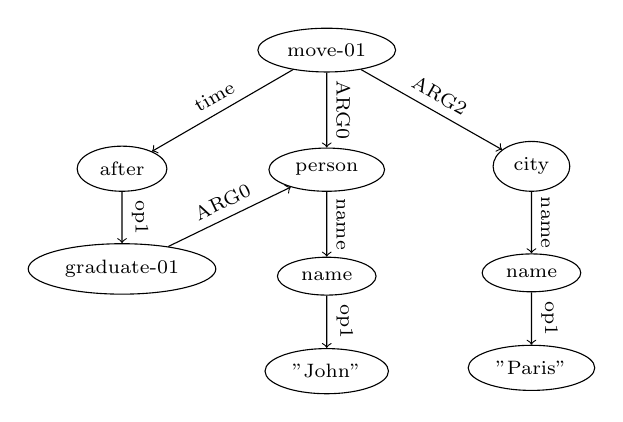
\begin{tikzpicture}[->,
      every node/.append style={sloped,anchor=south,auto=false,font=\scriptsize},
      level 1/.style={level distance=18mm,sibling distance=26mm},
      level 2/.style={level distance=16mm},
      level 3/.style={level distance=15mm}]
    \node (ROOT) [draw=black,ellipse] {move-01}
      child {node [draw=black,ellipse] {after}
      {
            child {node (graduation) [draw=black,ellipse] {graduate-01} edge from parent node {op1} }
      } edge from parent node {time} }
      child {node (John) [draw=black,ellipse] {person}
      {
        child {node [draw=black,ellipse] {name}
        {
            child {node [draw=black,ellipse] {"John"} edge from parent node {op1} }
        } edge from parent node {name} }
      } edge from parent node {ARG0} }
      child {node [draw=black,ellipse] {city}
      {
        child {node [draw=black,ellipse] {name}
        {
            child {node [draw=black,ellipse] {"Paris"} edge from parent node {op1} }
        } edge from parent node {name} }
      } edge from parent node {ARG2} }
      ;
      \draw (graduation) to node {ARG0} (John);
  \end{tikzpicture}
\caption{AMR graph.
  The text tokens are not part of the graph, and must be matched to
  concepts and constants by alignment.
  Variables are represented by their concepts.}
\label{fig:original_example}
\end{figure}


\section{Abstract Meaning Representation}\label{sec:amr}

AMR \cite{banarescu2013abstract}
is a semantic representation that embeds annotations related
to named entity recognition, semantic role labeling, word
sense disambiguation and co-reference resolution.
AMRs are rooted and directed graphs, in which both nodes and edges are labeled.
Most AMRs are DAGs, although cycles are permitted.
AMR was targeted in the SemEval 2017 shared task \cite{may2017semeval}.

As can be seen in Figure~\ref{fig:original_example}, text tokens are not part
of the AMR graph, which connects only concepts (from a pre-defined set)
and constants (which may be strings or numbers).
During the process of parsing from plain text to AMR,
the tokens are aligned to graph nodes,
a process referred to as concept identification.
AMR datasets already contain automatically aligned graphs.


\begin{figure}
  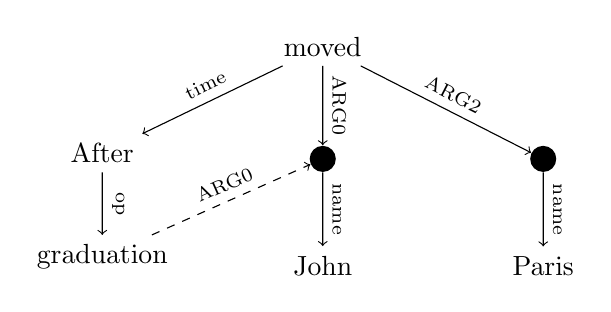
\begin{tikzpicture}[level distance=16mm, ->,
      every node/.append style={sloped,anchor=south,auto=false,font=\scriptsize},
      level 1/.style={sibling distance=28mm},
      level 2/.style={sibling distance=14mm},
      level 3/.style={sibling distance=12mm}]
    \tikzstyle{word} = [font=\rmfamily,color=black]
    \node (ROOT) [word] {moved}
      child {node [word] {After}
      {
            child {node (graduation) [word] {graduation} edge from parent node {op} }
      } edge from parent node {time} }
      child {node (John) [fill=black,circle] {}
      {
        child {node [word] {John} edge from parent node {name} }
      } edge from parent node {ARG0} }
      child {node [fill=black,circle] {}
      {
        child {node [word] {Paris} edge from parent node {name} }
      } edge from parent node {ARG2} }
      ;
      \draw[dashed] (graduation) to node {ARG0} (John);
  \end{tikzpicture}
\caption{Converted AMR graph, with
  text tokens added according to the alignments, and
  pre-terminals included to show node labels.
  The placeholders $\langle \ell \rangle, \langle v \rangle$ and $\langle T \rangle$
  correspond to the lemma, related verb form and surface form, respectively.
  Numeric suffixes of \textit{op} relations were removed,
  and names collapsed.}
\label{fig:converted_example}
\end{figure}


\section{DAG format}\label{sec:conversion}

\cite{hershcovich2018multitask}
In this format, the graph is a rooted DAG, and the text tokens are terminal nodes.
Edges are labeled, and nodes are optionally labeled too (to support AMR parsing).
All edges entering terminals bear the \textit{Terminal} label.
As in the UCCA format,
graph edges are divided into \textit{primary} and \textit{remote} edges,
where the primary edges form a tree (all nodes have at most one primary parent,
and the root has none).
The remote edges enable reentrancy, and thus together with them the graph
is in general a DAG and not necessarily a tree.
Not all non-terminals must have terminal descendants.
Non-terminals with an empty terminal yield are called \textit{implicit}.
Figure~\ref{fig:converted_example} shows examples for a converted graph.

In case of reentrancy, an arbitrary parent is marked as primary, and the rest as remote
(denoted as dashed edges in Figure~\ref{fig:converted_example}).

In the conversion from AMR, non-terminals are already present and do not need to be introduced.
However, alignments and node labels must be handled.

\subsection{Alignments}
Since alignment to the text tokens is not part of the AMR graph,
we introduce the alignments as edges in conversion.
We use automatically aligned AMR graphs provided in the dataset (see \S\ref{sec:data}),
and attach each node with a \textit{Terminal} edge to each of the terminals it is aligned to.

\subsection{Node label sparsity}
To reduce the number of unique node labels, we use the alignments to introduce
placeholders in the labels.
For example, a node labeled \textit{move-01} aligned to the terminal \textit{moved} will
be instead labeled $\langle \ell \rangle$\textit{-01},
where $\langle \ell \rangle$ is a placeholder for the token's lemma.
In this way we reduce the number of node labels in the dataset from tens of thousands to 7300,
of which 2000 occur only once and are treated as unknown.
We use similar placeholders for the token's text and capitalized text,
negation, verb, noun and adjective form
(from a pre-defined lexicon), and Wikipedia concept.
We use DBpedia Spotlight to wikify concepts \cite{isem2013daiber}.
In addition, we omit all variable identifiers and instead label nodes directly with their concept.
This is similar to the delexicalization employed by \citet{buys2017oxford}.

\subsection{Edge label sparsity}
Another sparsity issue is with ordinal relations, such as \textit{op1}, \textit{op2}, etc.
Since the order of relations is annotated according to the order of text tokens,
the numeric index is redundant and is thus removed.
We keep the numeric suffixes when they are meaningful, e.g. in \textit{ARG0}, \textit{ARG1}, etc.

\subsection{Names}
Named entities in AMR are expressed by \textit{name} relations and nodes, with
a child for each token in the name, with relations labeled \textit{op1}, \textit{op2}, etc.
We instead collapse this subgraph to a single node whose label is the concatenation of the
name tokens, replaced by a $\langle T \rangle$ placeholder if aligned.



\section{Transition-based universal parser}\label{sec:model}

The DAG format introduced in \S\ref{sec:conversion}
exhibits reentrancy, discontinuity and non-terminal nodes.
To learn to parse representations in this format,
we extend TUPA \cite{hershcovich2017a},
a transition-based parser that supports these structural properties,
originally developed for UCCA.
TUPA's general transition system allows parsing any aligned DAG structure with labeled edges.
To support AMR parsing, we add transitions to handle node labels and unaligned nodes
(see \S\ref{sec:transition_set}).

Transition-based parsers \cite{Nivre03anefficient} apply \textit{transitions}
incrementally to an internal state defined by
a buffer $B$ of remaining tokens and nodes,
a stack $S$ of incomplete nodes,
and a labeled graph $G$ of constructed nodes and edges.
When the parsing process is finished, the graph $G$ is the final output.
A classifier is used at each step to select the next transition based on features
encoding the current state.
During training, an oracle creates training instances for the classifier,
based on gold-standard annotations.


\subsection{Transition set}\label{sec:transition_set}
Given a sequence of tokens $w_1, \ldots, w_n$,
we predict a graph $G$ in the unified format over the sequence.
Parsing starts with the root node on the stack,
and the input tokens in the buffer.

The original TUPA transitions are
the standard \textsc{Shift} and \textsc{Reduce} operations,
\textsc{Node$_X$} for creating a new non-terminal node and an $X$-labeled edge,
\textsc{Left-Edge$_X$} and \textsc{Right-Edge$_X$} to create a new primary $X$-labeled edge,
\textsc{Left-Remote$_X$} and \textsc{Right-Remote$_X$} to create a new remote $X$-labeled edge,
\textsc{Swap} to handle discontinuous nodes,
and \textsc{Finish} to mark the state as terminal.

In addition, we add the \textsc{Implicit} transition, creating a new non-terminal
node as a \textit{child} of the current stack top rather than as its parent,
and transitions to
label nodes in the stack, \textsc{Label$_1$} and \textsc{Label$_2$},
labeling the stack top and one node to its left, respectively.

Although UCCA contains implicit units, that is, units without
any terminals as descendents,
the standard evaluation for UCCA \cite{abend2013universal} is span-based and
ignores these nodes.
For this reason we do not include this transition when parsing UCCA.
However, for AMR we do include it, as AMRs may contain unaligned concepts,
which correspond to implicit nodes in the unified format.
These are essential for AMR parsing, for which evaluation is done
by graph matching, using the Smatch algorithm \cite{cai2013smatch}.

The reason for including \textsc{Label$_2$} is that often a node's
label can be determined more accurately only after attaching its children,
which may require it to be the second node on the stack.
To keep the overall number of transitions manageable,
the node label itself is not part of the transition's identity,
instead being selected by a separate classifier.

\subsection{Classifier}\label{sec:classifier}
We experiment with two different models for the parser in the single-task case:
(1) a linear classifier with sparse features, trained with the averaged structured perceptron algorithm
\cite{Coll:04} and \textsc{MinUpdate} \cite{goldberg2011learning},
and (2) a bidirectional LSTM feature extractor with dense embeddings as inputs,
combined with a feedforward network and a softmax layer for classification.

For all classifiers, inference is performed greedily,
and training is done with an oracle that provides a set of all possible labels at a given state
(but only valid transitions may be taken during training).


\begin{figure}[t]
   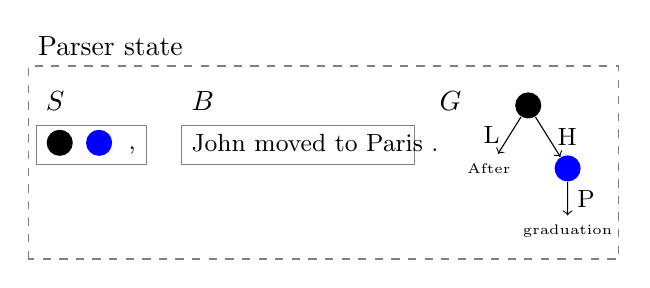
\begin{tikzpicture}[level distance=8mm, sibling distance=1cm]
   \node[anchor=west] at (0,1.5) {Parser state};
   \draw[color=gray,dashed] (0,-1.2) rectangle (7.5,1.25);
   \draw[color=gray] (.1,0) rectangle (1.5,.5);
   \node[anchor=west] at (.1,.8) {$S$};
   \node[fill=black, circle] at (.4,.275) {};
   \node[fill=blue, circle] at (.9,.275) {};
   \node[anchor=west] at (1.15,.175) {\small ,};
   \draw[color=gray] (1.95,0) rectangle (4.9,.5);
   \node[anchor=west] at (1.95,.8) {$B$};
   \node[anchor=west] at (1.95,.275) {\small John moved to Paris .};
   \node[anchor=west] at (5.1,.8) {$G$};
   \node[fill=black, circle] at (6.35,.75) {}
     child {node  {\tiny After} edge from parent [->] node[left] {\small L}}
     child {node [fill=blue, circle] {}
     {
       child {node {\tiny graduation} edge from parent [->] node[right] {\small P}}
     } edge from parent [->] node[right] {\small H} };
   \end{tikzpicture}
   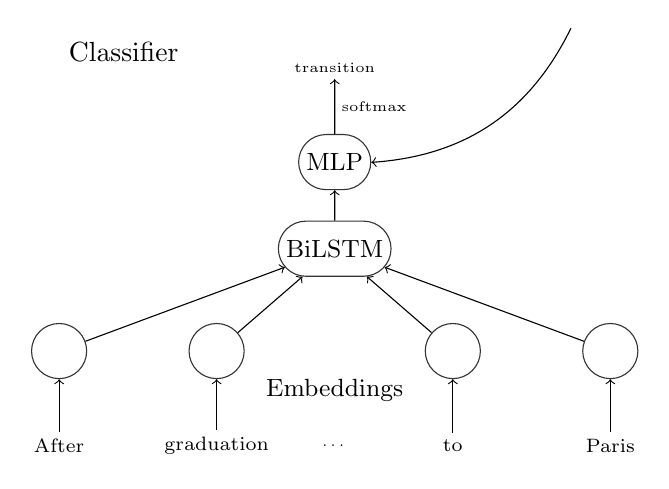
\begin{tikzpicture}[->]
   \node[anchor=west] at (0,6) {Classifier};
   \tiny
   \tikzstyle{main}=[rounded rectangle, minimum size=7mm, draw=black!80, node distance=12mm]
   \node[main] (specific) at (3.5,3.5) {\small BiLSTM};
   \node (embeddings) at (3.5,1.7) {\small Embeddings};
   \foreach \i/\word in {0/{After},2/{graduation},5/{to},7/{Paris}} {
       \node (x\i) at (\i,1) {\scriptsize \word};
       \node[main] (e\i) at (\i,2.2) {};
       \path (x\i) edge (e\i);
       \path (e\i) edge (specific);
   }
    \node (x4) at (3.5,1) {\ldots};
    \node[main] (mlp) at (3.5,4.6) {\small MLP};
    \path (specific) edge (mlp);
    \coordinate (state) at (6.5,6.3);
    \path (state) edge [bend left] (mlp);
    \node (transition) at (3.5,5.8) {transition};
    \path (mlp) edge node[right] {softmax} (transition);
   \end{tikzpicture}
\caption{Illustration of the TUPA model, from \citet{hershcovich2018multitask}.
Top: parser state.
Bottom: BiLTSM architecture.}\label{fig:single_model}
\end{figure}

In addition to the features used by \citet{hershcovich2017a},
for AMR we add node label features according to
previously predicted node labels for node in specific locations in the parser state.
All features are shared among all tasks, except the node labels, which are
AMR-specific.

Lemmas, POS tags, syntactic dependency labels and named entities are extracted using spaCy
\cite{spacy2}.\footnote{\url{https://spacy.io}}
We use the categorical cross-entropy objective function and optimize the
NN classifiers with stochastic gradient descent (SGD).
We use 250K word vectors from fastText \cite{bojanowski2016enriching}, pretrained over Wikipedia.
The neural network is implemented using DyNet \cite{neubig2017dynet}.\footnote{\url{https://dynet.io}}
Hyperparameter settings are listed in Table~\ref{tab:hyperparams}.

\begin{table}
\begin{tabular}{l|ccccc}
\hline
\footnotesize Dimensions &  main & aux & shared \\
\hline
external word & & & 300 \\
word & & & 200 \\
POS tag & & & 20 \\
syntactic dep. & & & 10 \\
punctuation & & & 1 \\
action & & & 3 \\
node label & & 20 \\
edge label & 20 \\
MLP \#layers & 2 & 2 \\
MLP layer dim. & 50 & 50 \\
LSTM \#layers & 2 & 2 & 2 \\
LSTM layer dim. & 500 & 50 & 500 \\
\hline\hline
\footnotesize Other parameters & Sparse & NN \\
\hline
$\textsc{MinUpdate}$ & 5 \\
initial learning rate & 1 & 1 \\
learning rate decay & 0.1 & 0.01 \\
word dropout & & 0.2 \\
dropout & & 0.4 \\
weight decay & & $10^{-5}$ \\
mini-batch size & & 100
\end{tabular}
\caption{Hyperparameter settings.\label{tab:hyperparams}}
\end{table}


\subsection{Constraints}

As each annotation scheme has different constraints on the allowed graphs,
we defined these constraints separately for each task.
During training and parsing, the constraint set corresponding to the task is
selected and applied to the parser state.

Some constraints are task-specific, while some are generic.
In AMR, a concept corresponding to a PropBank frame may have only core arguments defined for the frame.

As an example for a generic constraint, nodes that have already been swapped
should never be swapped again.
To implement this constraint efficiently, we define a \textit{swap index}
for each node, which is assigned when the node is created.
At parse start, only the root node and terminals exist.
We assign the root a swap index of 0, and for each terminal, its swap index
is its position in the text (starting at 1).
Whenever a node is created as a result of a \textsc{Node} or \textsc{Implicit}
transition, we assign its swap index to be the mean of the stack top and buffer
head's swap indices.


\section{Multitask transition-based parsing}\label{sec:multitask}

Since the same model can be applied to different tasks, we can train it jointly on multiple tasks.
In this section we focus on the NN model.
Rather than sharing the whole set of parameters (and getting a mix of action labels as a result),
we share only part of the model.
Specifically, in addition to the task-specific input-encoding bidirectional LSTM,
we use a shared bidirectional LSTM. The outputs of both LSTMs are concatenated and
fed into the task-specific MLP (see Figure~\ref{fig:model}),
in a manner similar to \citet{P17-1186}.


\section{Experiments}\label{sec:experiments}


\subsection{Data}\label{sec:data}

For AMR, we use LDC2016E25, used in SemEval 2017 \cite{may2017semeval}.

\begin{table}
\begin{tabular}{lcc}
Corpus & \# Tokens & \# Sentences \\
\textbf{UCCA} \\
\textbf{AMR} \\
LDC2016E25 & 708701 & 39260 \\
\end{tabular}
\caption{Size of each corpus.\label{tab:corpora}}
\end{table}


\subsection{Evaluation}\label{sec:evaluation}

For AMR, we use Smatch \cite{cai2013smatch}.


\subsection{Results}\label{sec:results}


The results when evaluated on the development set are shown in Table~\ref{tab:single}.


\begin{table}
\begin{tabular}{llccc}
\textbf{AMR \small(LDC2016E25)} & \small Smatch & \textbf{P} & \textbf{R} & \textbf{F1} \\
Sparse & & 55 & 53.7 & 54.4 \\
NN & & 66.7 & 64.7 & 65.7 \\
\multicolumn{4}{l}{\citet{foland2017abstract}} & 70.9 \\

\end{tabular}
\caption{Results on dev set.
Best reported results given for comparison.
\label{tab:single}}
\end{table}




\section{Related work}\label{sec:related_work}

\cite{wang2015transition,damonte-17}

\section{Discussion}\label{sec:discussion}


\bibliography{references}
\bibliographystyle{acl_natbib}

\end{document}
